\documentclass[../main/Feedback.tex]{subfiles}
\begin{document}
\section{Results}
Beyond using the SAM to monitor for ethical concerns whilst participants viewed footage of car crashes, we used this data to check that the videos could be considered comparable. 
There was no statistical significance as assessed by Friedman between the three videos for SAM emotional valence and arousal.
Overall, based on post-study ratings, the bulk of participants preferred index1 and index3 with 8 and 6 votes respectively compared to index2 which was preferred by 3 participants. 
There was also no significant difference, however, in the mean time to complete the task in each web form condition ($F(2,28)=0.498, p<0.613$), nor the emotional valence associated with the three web forms ($X^{2}(2)=5.15,p=0.076$). 
Instead, below we examine our measures of MWL for a difference between conditions.
\subsection{Objective Mental Workload - fNIRS}
A one-way repeated measures ANOVA test found a significant difference in the mean levels of Hbo between the 3 web forms ($F(2,22)=4.324, p<.026,$ partial $\eta^{2}=.282$), as shown in Figure ~\ref{fig:mean-hbo-index123}. 
The assumption of sphericity was met, as assessed by Mauchly's test of sphericity, $X^{2}(2) = 0.975, p = 0.879$. 
The measured mean Hbo was \textit{higher} for index3 0.644 (SD = 1.37) compared to both index2 0.384 (SD = 1.28) and index1 0.139 (SD = 1.21). 
A Post hoc analysis with a Bonferroni adjustment revealed that the difference in HbO between index3 and index 1 was significantly higher compared to index1, $p=0.047$.

\begin{figure}[h]
	\centering
	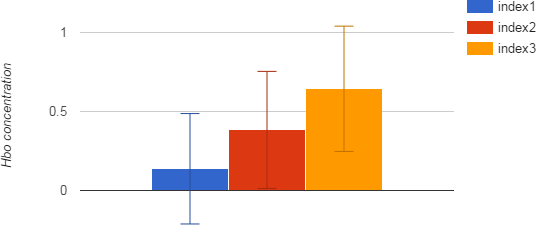
\includegraphics[width=1\linewidth]{../figures/mean-Hbo-concentration-index123}
	\caption[mean Hbo activation between the three web forms]{Mean Hbo activation between the three web form conditions as measured by fNIRS. Higher Hbo values indicates higher workload.}
	\label{fig:mean-hbo-index123}
\end{figure}
		
%		\begin{figure}[h]
%			\centering
%			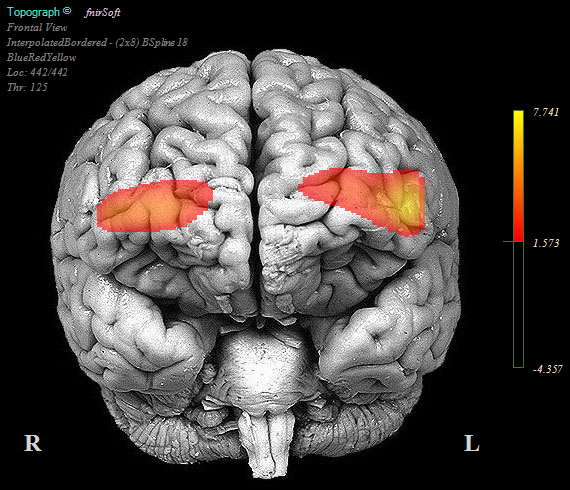
\includegraphics[width=0.7\linewidth]{../figures/p2-index3-brain-view-left-activation}
%			\caption[Brain view of Participant's 2 Hbo activation during web form filling of index3]{Brain view of Participant's 2(P2) Hbo activation during web form filling of index3. It can be noted more hemodynamic activation in the left hemisphere. P2 rated its emotional valence as positive (4/5).}
%			\label{fig:p2-index3-brain-view-left-activation}
%		\end{figure}
		
%		\begin{figure}[h]
%			\centering
%			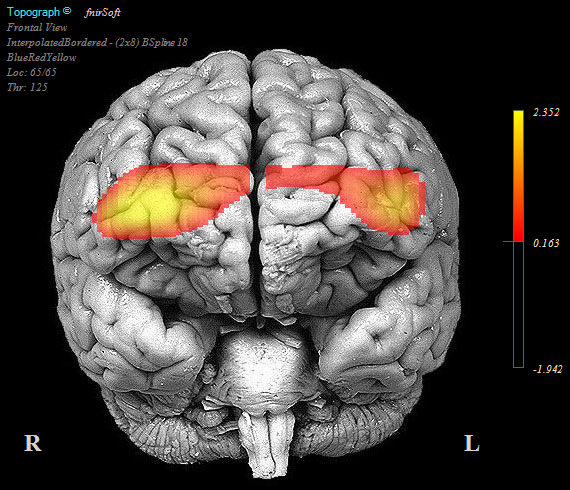
\includegraphics[width=0.7\linewidth]{../figures/p2-video3-brain-view}
%			\caption[Brain view of Participant 2 while viewing video of road accident(video3)]{Brain view of Participant 2 while viewing video of road accident(video3). More arousal can be noted and more right hemisphere activation, which is expected as automotive accidents increase arrousal and emotional state becomes negative.}
%			\label{fig:p2-video3-brain-view}
%		\end{figure}
\subsection{Subjective Mental Workload - NASA-TLX}
There was significant statistical difference between the three web forms in the perceived mental demand $F(2,28)=4.677, p<.018$ partial $\eta^{2}=.250$ score as assessed by one way repeated measures ANOVA. 
Inline with the objective data from the fNIRS, participants perceived index3 as the most mentally demanding with mean score of 11.87 (SD = 5.04), followed by index2 with 9.67 (SD = 5.02) and index3 8.73 (SD = 4.41).
Post hoc analysis with Bonferonni correction revealed significant interaction between index1 and index3 with $p=0.018$.
		%Also, the time to complete index1 and index3 had a strong positive correlation with perceived mental demand (NASA-TLX) for index1 and index3: $r(13)=0.546, p=0.035$ and $r(18)=0.649, p=0.009$. However, time to complete index2 does not correlate to perceived mental demand of index2 $r(18)=0.472, p=0.076$.
		
%		\begin{table}[h]
%			\centering
%			\caption[NASA-TLX mean scores]{A table of all of the calculated mean NASA-TLX values for the 6 subscales, including the averaged total tlx}
%			\label{nasa-tlx}
%			\begin{tabular}{l|ccc}
%				& Index1           & Index2           & Index3           \\[0.12cm]   \hline
%				Mental demand   & 9.15 (SD = 4.94) & 9.40 (SD = 4.68) & 10.8 (SD = 5.38) \\
%				Physical demand & 4.05 (SD = 4.08) & 2.90 (SD = 3.21) & 3.90 (SD = 3.65) \\
%				Temporal demand & 7.40 (SD = 4.49)  & 7.65 (SD = 5.79) & 6.55 (SD = 4.91) \\
%				Performance     & 6.65 (SD = 3.79) & 5.60 (SD = 3.62)  & 6.20 (SD = 3.86)  \\
%				Effort          & 8.15 (SD = 4.58) & 7.35 (SD = 4.68) & 8.20 (SD = 5.30)   \\
%				Frustration     & 6.10 (SD = 5.11)  & 6.00 (SD = 3.66)  & 6.75 (SD = 5.22) \\\hline
%				Total 			& 6.92 (SD = 2.95) & 6.47 (SD = 3.11) & 7.07 (SD = 3.22)
%			\end{tabular}
%		\end{table}
%		

		
%		\begin{figure}[h]
%			\centering
%			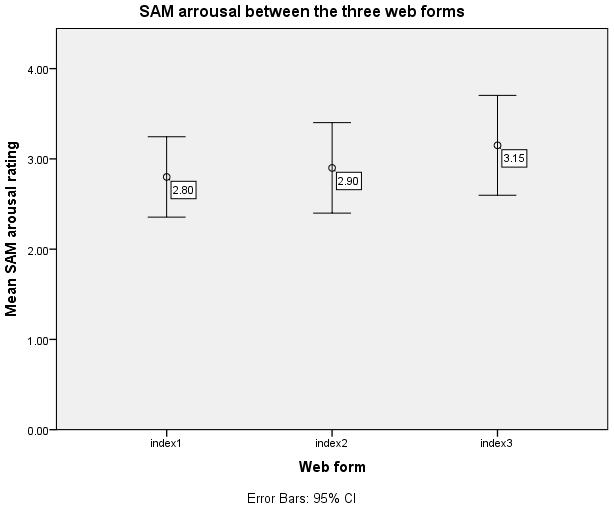
\includegraphics[width=0.7\linewidth]{../figures/sam-arrousal-index123}
%			\caption[SAM arrousal between the three web forms]{The mean SAM arrousal rating obtained from the three web form conditions.}
%			\label{fig:sam-arrousal-index123}
%		\end{figure}
		
%		\subsection{Emotional Valence and Arousal (SAM)}
%		\subsubsection{Data from the period of web form filling}
%		There was no significant statistical difference in the SAM emotional valence scale between the 3 web forms $X^{2}(2)=5.15,p=0.076$ as assessed by Friedman test.
%		The perceived mean emotional valence for index1 was the lowest with 3.07 (SD = 0.96) increasing to 3.33 (SD = 1.05) for index2 and to 3.67 (SD = 0.90) for index3.
%		However, the median for index3 was highest with 4, compared to index1 and index2 which had a median 3.
%		
%		% as it can be seen from Figure \ref{fig:sam-valence-index123}.
%%		\begin{figure}[h]
%%			\centering
%%			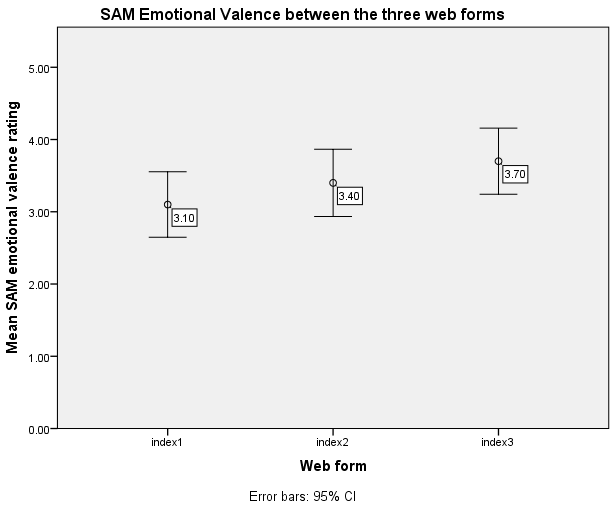
\includegraphics[width=0.7\linewidth]{../figures/sam-valence-index123}
%%			\caption[emotional valence between the 3 conditions]{Perceived emotional valence between the 3 web form conditions}
%%			\label{fig:sam-valence-index123}
%%		\end{figure}
%		The perceived arousal was lowest for index1 2.73 (SD = 1.03) increasing to 2.80 (SD = 1.08) for index2 and to 3.13 (SD = 1.36) for index3 respectfully. No statistical significance was found when comparing the three conditions.

%		\subsection{Task completion time}		
%		The mean time to complete index1 was the lowest 216.78 (SD = 61.60) increasing to 221.35 (SD = 67.26) for index2 and to 235.19 (SD = 86.46) for index3. However,
%		There was no significant statistical difference between the 3 web forms $F(2,28)=0.498, p<0.613$ partial $\eta^{2}=.034$, as assessed by one-way repeated measures ANOVA.
%		\subsection{User preferences from the short-interview question}
%		\begin{figure}[h]
%			\centering
%			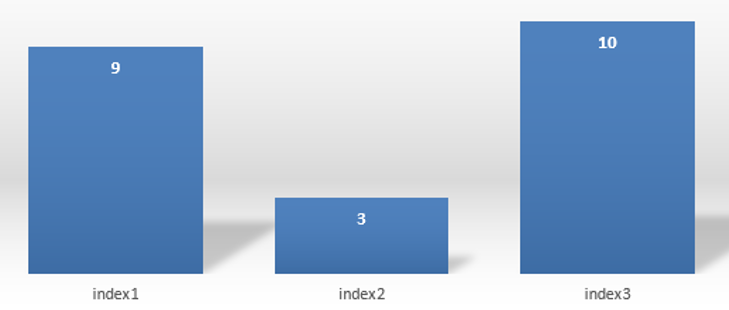
\includegraphics[width=0.7\linewidth]{../figures/user-preferences}
%			\caption[Participant preferences]{At the end of the experiements participants were asked which of the 3 web forms they preferred the most. Th sum of the amswers is depicted in a bar chart.}
%			\label{fig:user-preferences}
%		\end{figure}			
\end{document} 